\subsection{Classification and Regression Trees}
\label{sec:CART}
The next 3 approaches all use a specific type of machine learning strategy to construct their predictors. This method is call Classification and Regression Tree's (\CART). These trees are typically binary trees that divide the given data points into small enough groups so a direct local prediction can be done. These local prediction are then combined into a global predictor \cite{VariabilityAwarePerformancePredictionJianmeiSigmundApel}. In the context of configurable software systems each point consists at least out of a configuration and an associated performance score. These data point are then fed into the algorithm seen in \cref{alg:CART}.

The node impurity found in the algorithm is typically calculated by the square mean error. To prevent \textit{under}- or \textit{overfitting}\cite{ElementsOfStatisticalLearning} the recursive splitting has to be stopped at the right time. This is possible by manual parameter tuning or using an empirical-determined automatic terminator. The size of the predictor variables set $X$ is usually 1. This means, that we decide the branching based on whether a feature is selected or not (or based on its value).
\setlength\intextsep{0pt}
\begin{figure}[t]
	\lstset{
		mathescape,
		breaklines=true,
	}
	\begin{lstlisting}
	1. Start at the root node. Assign all configurations to it.
	2. For each option, find the set of options $X$ that minizes the sum of the node impurities in the two child nodes. Divide the configurations assigned to the current node based on $X$ into two disjoint sets and assign those to the corresponding child nodes.
	3. If a stopping criterion is reached, exit. Otherwise, apply step 2 and 3 to each child node inturn.
	\end{lstlisting}
	\captionof{lstlisting}{Pseudocode for generating a \CART. Adopted from \citet{ClassificationAndRegressionTrees} to fit software configurations.}
	\label{alg:CART}
\end{figure}
When using the \CART~found in \cref{fig:VAPPExampleTree}a configuration $c=\{\dots,\;x_3=1,\;\dots,\;x_{14}=0,\;x_{15}=0,\;\dots\}$ would be classified as $S_{RRL}$. The predicted performance of this class and therefore for $c$ is $\ell_{S_{RRL}}=571$.

\begin{figure}
	\centering
	\includegraphics[page=4,clip,trim=3.5cm 18cm 3.5cm 1.5cm, width=11.625cm]
	{Paper/VariabilityAwarePerformancePredictionAStatisticalLearningApproach.pdf}
	\caption{Example performance model of X264 generated by CART based on the random sampling (N=16), using minimization of the sum of squared error loss \cite{VariabilityAwarePerformancePredictionJianmeiSigmundApel}.}	
	\label{fig:VAPPExampleTree}	
\end{figure}
\noindent
\FloatBarrier